\chapter{Analyse des résultats}

\index{résultats}
\section{Présentation des résultats}
Les résultats de la mesures des frquence dans de plusieurs milieux sont présentés dans la figure \ref{fig:Réponse frequencielle amplitude}.
les milieux sont l'air, l'eau, l'ethanol et l'huile moteur. Chaqun de ces composant a une viscosité différente. 
Il est evident que non seulement la fréquence de pick mais égalment l'amplitude de chaque echantillon change. 
\begin{figure}[H]
    \centering
    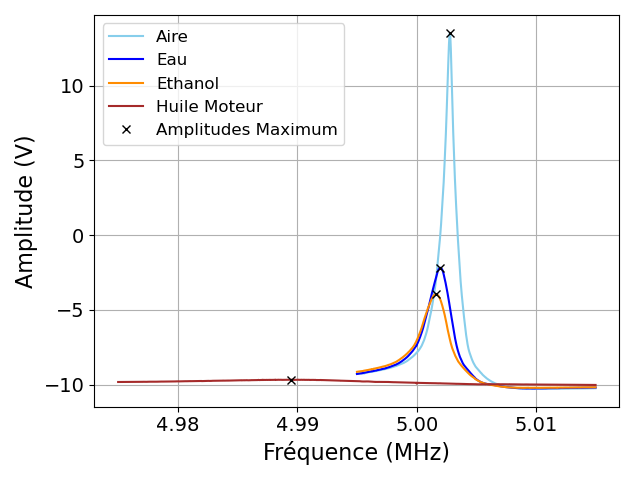
\includegraphics[width=\textwidth]{assets/figures/reponseFrequence.png}
    \caption{Réponse frequencielle du capteur selon plusieurs milieux}
    \label{fig:Réponse frequencielle amplitude}
\end{figure}

\begin{figure}[H]
    \centering
    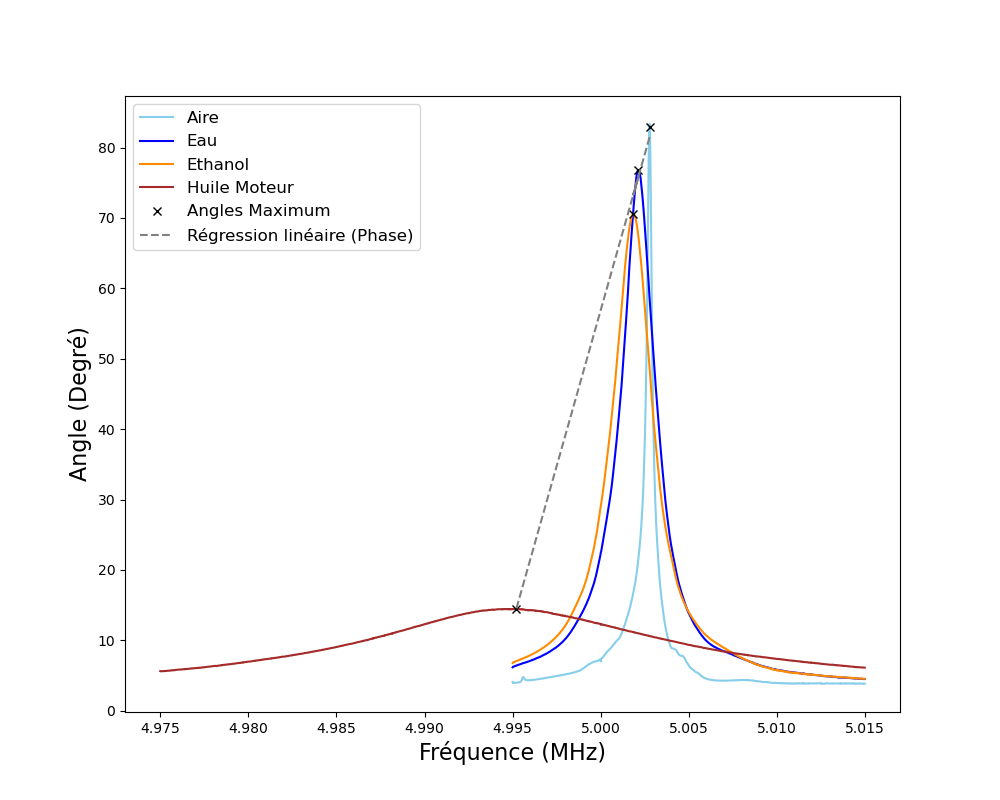
\includegraphics[width=\textwidth]{assets/figures/reponsePhase.png}
    \caption{Réponse frequencielle de déphasage du capteur selon plusieurs milieux}
    \label{fig:Réponse frequencielle déphasage}
\end{figure}


\subsection{Gelification}
Les resultat de la mesure de la gelification sont présentés dans la figure \ref{fig:Frequence gelification}. 
Lorsque le liquide est refroidi,
un chagement de la pente entre de la fréquence de résonance et la température est visible au environ des 25°C, 
en dessus de cette temperature la pente est similaire à celle de l'eau. en dessous la pente est plus importante.  
Ce changement indiquerais un changement de l'état du gel. Passant de l'état liquide à l'état gélifié.
Une fois que le liquide à attein ca temérature minimal et que de l'eau chaude circule autour du capteur,
la temperature augment plus vite que la fréquance de raisonnance. un autre point de chacngement de phase est visible au environ de 32°C ce qui corrresponderais à la temperature de liquefaction de la gélatine en liquide.
\begin{figure}[H]
    \centering
    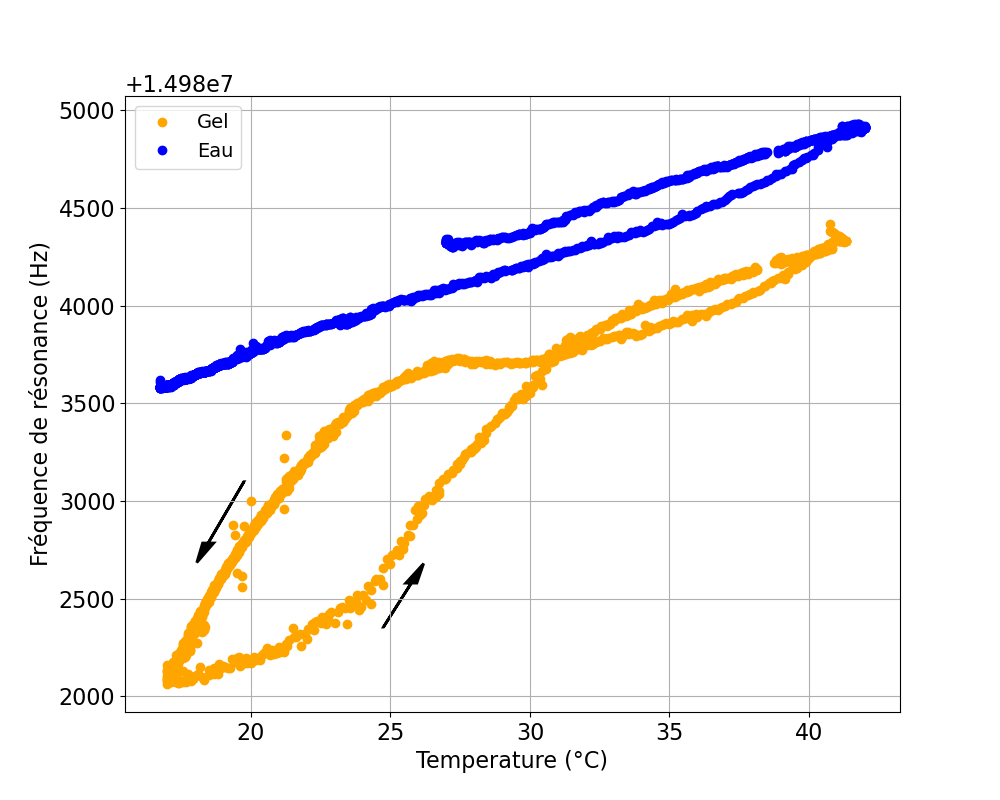
\includegraphics[width=\textwidth]{assets/figures/gel.png}
    \caption{Frequence de résonance en fonction de la temperature pour la mesure de la gelification}
    \label{fig:Frequence gelification}
\end{figure}
\section{Discussion des résultats}

La discussion constitue une étape essentielle, car elle vous permet de donner du sens à vos résultats. Vous devez aller au-delà de la simple présentation des données en les analysant de manière critique et en les confrontant aux travaux existants.

Cette section doit permettre :
\begin{itemize}
    \item De comparer vos résultats à ceux issus de la littérature ou d'études antérieures, afin de mettre en perspective vos observations.
    \item D'évaluer la pertinence de vos résultats et d'en discuter les implications théoriques ou pratiques.
    \item De justifier les résultats obtenus, en expliquant les causes potentielles des écarts observés ou des résultats inattendus.
    \item D'identifier les limites de votre étude et d'en proposer des pistes d'amélioration pour de futurs travaux.
\end{itemize}

Cette réflexion critique démontre votre capacité à analyser vos résultats de manière approfondie et à en tirer des enseignements pertinents. Elle est essentielle pour montrer que vous maîtrisez non seulement vos données, mais également les implications qu'elles soulèvent dans le cadre de votre recherche.
